\section{Limpando a Poluição na Web: O Navegador Brave \faShield*}

A Web que usamos hoje não é gratuita; nós pagamos por ela com os nossos dados. Navegadores tradicionais (como Chrome ou Edge) foram projetados para rastrear o que você pesquisa, quanto tempo você olha para uma imagem e o que você pretende comprar. 

\vspace{0.3cm}
Como vimos em nossa oficina, o problema não são apenas os \enquote{biscoitos} (cookies) que você aceita. Hoje, as empresas usam técnicas avançadas chamadas de \textit{Fingerprinting} (Impressão Digital do Dispositivo). Elas olham o tamanho da sua tela, a marca do seu celular e a sua bateria para saber quem você é, mesmo no \enquote{Modo Anônimo}.

\vspace{0.3cm}
A solução para isso não é parar de navegar pela Web, mas sim usar um \textbf{Escudo Ativo}: o navegador \textbf{Brave}.

\vspace{0.3cm} % Respiro
\begin{figure}[h]
	\centering
	
\includegraphics[width=0.2\textwidth]{imagens/brave_logo.png}
	\caption*{(\citeauthor{brave_app} \citefield{brave_app}{version} - Versão oficial)}
\end{figure}

\subsection*{Por que usar o Brave no dia a dia?}

\begin{itemize}
	\item \textbf{Bloqueio Nativo de Anúncios:} Ele remove propagandas chatas de sites e vídeos do YouTube automaticamente.
	\item \textbf{Navegação Web mais Rápida:} Como o celular não precisa baixar os \enquote{espiões} e os banners de propaganda, os sites carregam até 3x mais rápido, economizando a sua franquia de dados 4G.
	\item \textbf{Não requer ser um gênio da informática:} Você não precisa instalar extensões difíceis. É só baixar e usar. O Brave bloqueia as invasões \enquote{de fábrica}.
\end{itemize}

\subsection*{Passo a Passo para Limpar sua Navegação:}

\begin{enumerate}
	\item Abra a loja de aplicativos do seu celular (Play Store ou App Store) e pesquise por \textbf{Brave Browser}. Para facilitar, você pode simplesmente \textbf{tocar nas imagens abaixo} (se estiver lendo no celular) ou \textbf{escanear o QR Code} com a câmera para ser levado direto ao aplicativo oficial.
	
	\vspace{0.3cm} % Respiro
	\begin{center} % Centraliza o bloco inteiro em relação à margem da lista
		\begin{minipage}{\linewidth} % Usa linewidth para não vazar a margem direita
			
			\begin{minipage}{0.3\linewidth}
				\centering
				\textbf{\textcolor{BraveOrange}{\faAndroid \ Android}}\\[0.2cm]
				\href{https://bfaxke.short.gy/brave-browser-android}{
					
\includegraphics[width=0.8\linewidth]{imagens/qr_brave_android.png}
				}\\[0.1cm]
				{\scriptsize (Toque ou escaneie)}
			\end{minipage}
			\hfill % Espaço flexível entre Android e iOS
			\begin{minipage}{0.3\linewidth}
				\centering
				\textbf{\textcolor{NordText}{\faApple \ iOS / iPhone}}\\[0.2cm]
				\href{https://bfaxke.short.gy/brave-browser-ios}{
					
\includegraphics[width=0.8\linewidth]{imagens/qr_brave_ios.png}
				}\\[0.1cm]
				{\scriptsize (Toque ou escaneie)}
			\end{minipage}
			\hfill % Espaço flexível entre iOS e Computador
			\begin{minipage}{0.3\linewidth}
				\centering
				\textbf{\textcolor{BitwardenBlue}{\faDesktop \ Computador}}\\[0.2cm]
				\href{https://bfaxke.short.gy/brave-desktop}{
					
\includegraphics[width=0.8\linewidth]{imagens/qr_brave_desktop.png}
				}\\[0.1cm]
				{\scriptsize (Para Windows/Linux/Mac)}
			\end{minipage}
			
		\end{minipage}
	\end{center}
	
	\item Instale o aplicativo \textbf{Brave} (o do Leão Laranja). 
	\item Ao abrir pela primeira vez, ele perguntará se deseja torná-lo seu \enquote{Navegador Padrão}. Escolha \textbf{Sim} (ou \enquote{Definir como padrão}). Isso garante que, ao clicar em um link no WhatsApp, você já abra protegido.
	\item \textbf{Pronto!} Agora, sempre que for pesquisar algo, ler notícias ou abrir o YouTube, use o Brave. 
\end{enumerate}

\subsubsection*{Usando a Funcionalidade Bloqueio de Elementos Integrada ao Navegador Brave}

Assim como as principais vantagens de privacidade do Brave, essa funcionalidade já vem nativamente integrada ao navegador. Você não precisa instalar extensões ou \textit{plugins} de terceiros, que frequentemente tornam a navegação mais lenta e abrem brechas de segurança \cite{Brave2026}. Vejamos como usá-la no Android.

\vspace{0.3cm}
Após instalar o aplicativo, acesse uma página de sua preferência --- neste exemplo, utilizamos o portal \textit{Minijogos} \cite{Minijogos2026}. Imediatamente ao abrir um site com perfil invasivo como este, o Brave inicia o bloqueio proativo de \textit{scripts} e \textit{cookies}. É crucial entender que, embora os sites aleguem que esses arquivos servem apenas para \enquote{funcionalidades}, a grande maioria atua como rastreadores silenciosos (\textit{trackers}), coletando dados sobre o seu dispositivo e hábitos de navegação \cite{NIST2025}.

\vspace{0.5cm} % Respiro

% --- BLOCO DE IMAGENS 1 (Passos 1 e 2) ---
\noindent % Para não dar recuo
\begin{minipage}{\textwidth}
	\centering
	\begin{minipage}{0.45\textwidth}
		\centering
		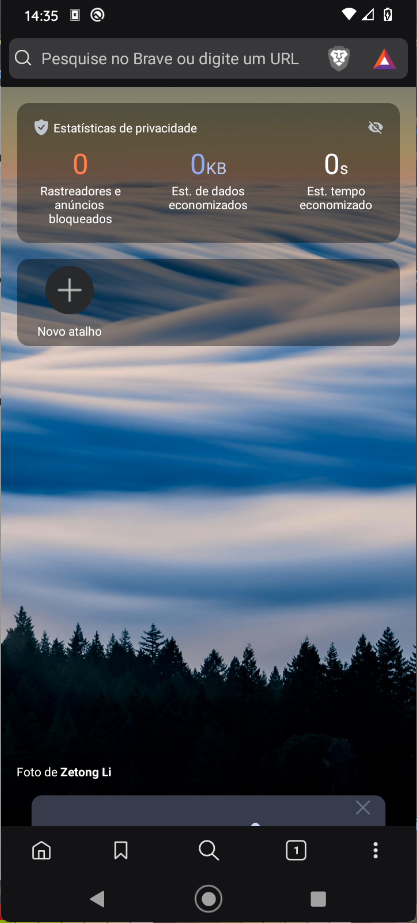
\includegraphics[trim={0cm 15cm 0cm 0cm}, clip, width=\textwidth]{imagens/brave_bloqueio_elementos_01.png}\\[0.2cm]
		\textbf{\textcolor{BraveOrange}{\faMobile* \ Passo 1}}
	\end{minipage}
	\hfill
	\begin{minipage}{0.45\textwidth}
		\centering
		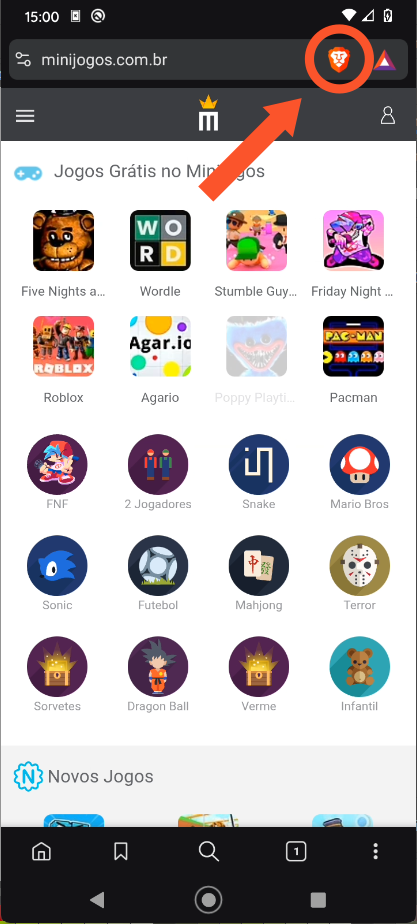
\includegraphics[trim={0cm 15cm 0cm 0cm}, clip, width=\textwidth]{imagens/brave_bloqueio_elementos_02.png}\\[0.2cm]
		\textbf{\textcolor{BraveOrange}{\faMobile* \ Passo 2}}
	\end{minipage}
\end{minipage}

\vspace{0.5cm} % Respiro
\noindent
\begin{minipage}{\textwidth}
	\textcolor{BraveOrange}{\textbf{Passo 1:}} Abra a página inicial\newline
	\textcolor{BraveOrange}{\textbf{Passo 2:}} Clique no ícone do \enquote{Leãozinho}
\end{minipage}
\vspace{0.3cm}

Assim, efetuado o Passo 2, abrirá uma aba (ou menu?) de opções abaixo do ícone do \enquote{Leãozinho}. Siga os passos abaixo.

\vspace{0.5cm}
% --- BLOCO DE IMAGENS 2 (Passos 3 e 4) ---
\noindent
\begin{minipage}{\textwidth}
	\centering
	\begin{minipage}{0.45\textwidth}
		\centering
		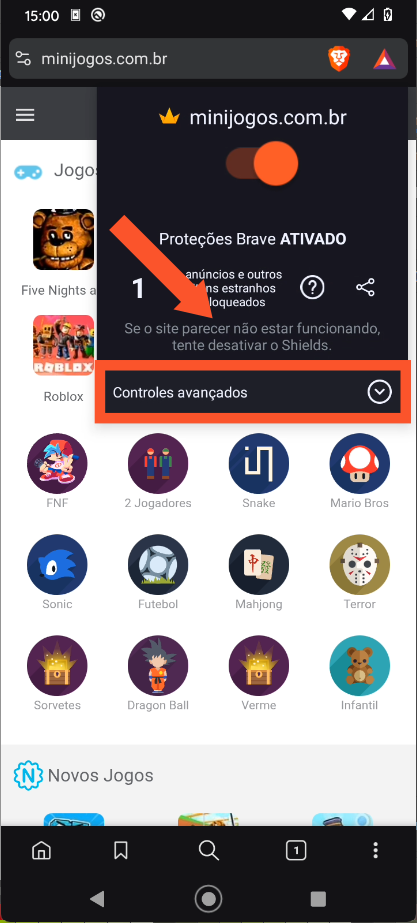
\includegraphics[trim={0cm 0cm 0cm 0cm}, clip, width=\textwidth]{imagens/brave_bloqueio_elementos_03.png}\\[0.2cm]
		\textbf{\textcolor{BraveOrange}{\faMobile* \ Passo 3}}
	\end{minipage}
	\hfill
	\begin{minipage}{0.45\textwidth}
		\centering
		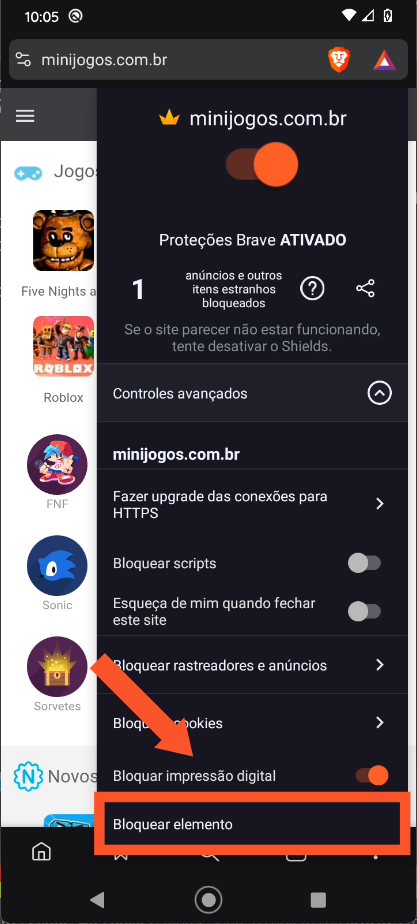
\includegraphics[trim={0cm 0cm 0cm 0cm}, clip, width=\textwidth]{imagens/brave_bloqueio_elementos_04.png}\\[0.2cm]
		\textbf{\textcolor{BraveOrange}{\faMobile* \ Passo 4}}
	\end{minipage}
\end{minipage}
% AdguardGreen

\vspace{0.5cm} % Respiro
\noindent
\begin{minipage}{\textwidth}
	\textcolor{BraveOrange}{\textbf{Passo 3:}} Clique em \enquote{Controles avançados}\newline
	\textcolor{BraveOrange}{\textbf{Passo 4:}} Clique em \enquote{Bloquear elemento}
\end{minipage}

\vspace{0.5cm}
% --- BLOCO DE IMAGENS 2 (Passos 3 e 4) ---
\noindent
\begin{minipage}{\textwidth}
	\centering
	\begin{minipage}{0.45\textwidth}
		\centering
		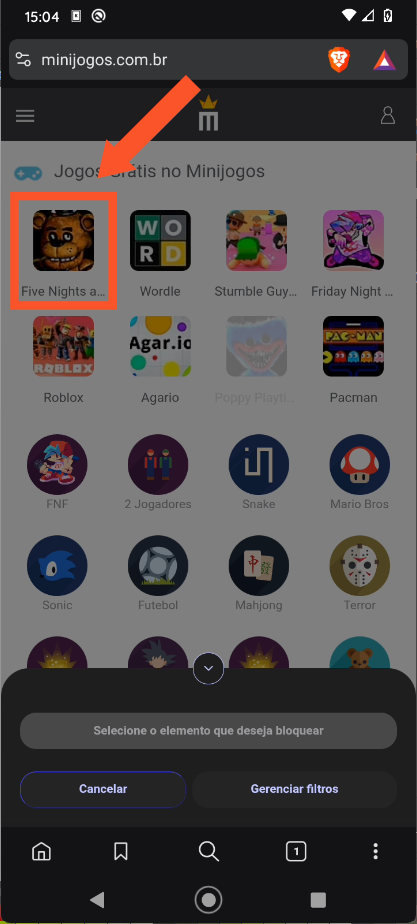
\includegraphics[trim={0cm 0cm 0cm 0cm}, clip, width=\textwidth]{imagens/brave_bloqueio_elementos_05.png}\\[0.2cm]
		\textbf{\textcolor{BraveOrange}{\faMobile* \ Passo 5}}
	\end{minipage}
	\hfill
	\begin{minipage}{0.45\textwidth}
		\centering
		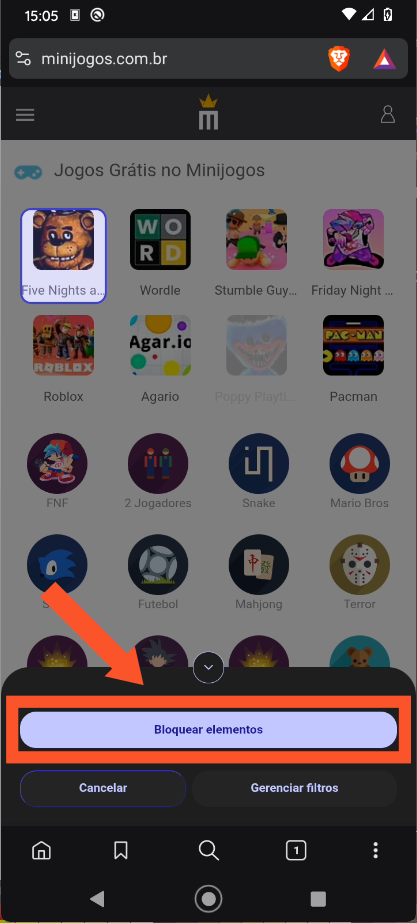
\includegraphics[trim={0cm 0cm 0cm 0cm}, clip, width=\textwidth]{imagens/brave_bloqueio_elementos_06.png}\\[0.2cm]
		\textbf{\textcolor{BraveOrange}{\faMobile* \ Passo 6}}
	\end{minipage}
\end{minipage}
% AdguardGreen

\vspace{0.5cm} % Respiro
\noindent
\begin{minipage}{\textwidth}
	\textcolor{BraveOrange}{\textbf{Passo 5:}} Escolha, por exemplo, o elemento \enquote{Five Nights a...}\newline
	\textcolor{BraveOrange}{\textbf{Passo 6:}} Clique em \enquote{Bloquear elementos}
\end{minipage}
\vspace{0.3cm}

\noindent
Parabéns! Você está livre do elemento \enquote{Five Nights a...}.
\vspace{0.3cm}

E se você se arrepender, e quiser o elemento de volta? Siga os passo abaixo para desfazer essa ação.

\vspace{0.5cm}
% --- BLOCO DE IMAGENS 2 (Passos 3 e 4) ---
\noindent
\begin{minipage}{\textwidth}
	\centering
	\begin{minipage}{0.45\textwidth}
		\centering
		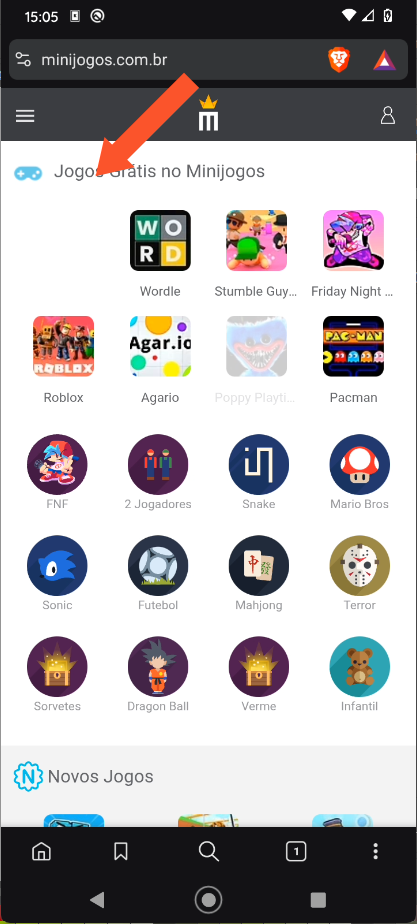
\includegraphics[trim={0cm 15cm 0cm 0cm}, clip, width=\textwidth]{imagens/brave_bloqueio_elementos_07.png}\\[0.2cm]
		\textbf{\textcolor{BraveOrange}{\faMobile* \ Passo 7}}
	\end{minipage}
	\hfill
	\begin{minipage}{0.45\textwidth}
		\centering
		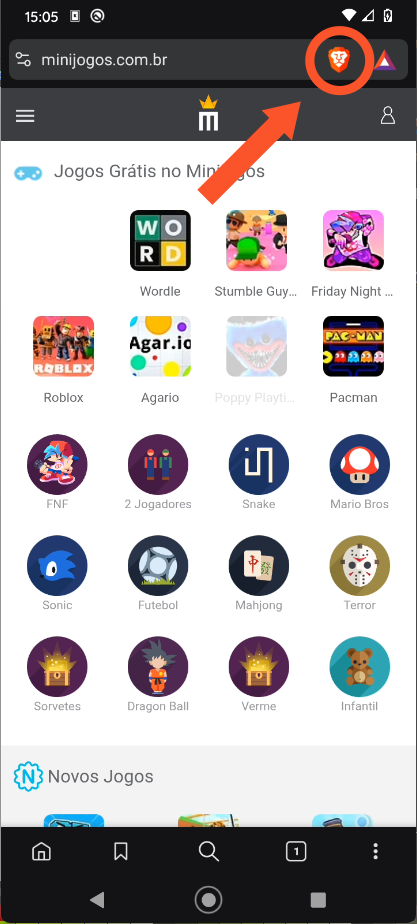
\includegraphics[trim={0cm 15cm 0cm 0cm}, clip, width=\textwidth]{imagens/brave_bloqueio_elementos_08.png}\\[0.2cm]
		\textbf{\textcolor{BraveOrange}{\faMobile* \ Passo 8}}
	\end{minipage}
\end{minipage}
% AdguardGreen

\vspace{0.5cm} % Respiro
\noindent
\begin{minipage}{\textwidth}
	\textcolor{BraveOrange}{\textbf{Passo 7:}} De fato, o elemento \enquote{Five Nights a...} sumiu\newline
	\textcolor{BraveOrange}{\textbf{Passo 8:}} Então, clique novamente no ícone do \enquote{Leãozinho}.
\end{minipage}
\vspace{0.3cm}

Abaixo do ícono do \enquote{Leãozinho}, o menu (a aba?) suspenso abrirá novamente:

\vspace{0.5cm}
% --- BLOCO DE IMAGENS 2 (Passos 3 e 4) ---
\noindent
\begin{minipage}{\textwidth}
	\centering
	\begin{minipage}{0.45\textwidth}
		\centering
		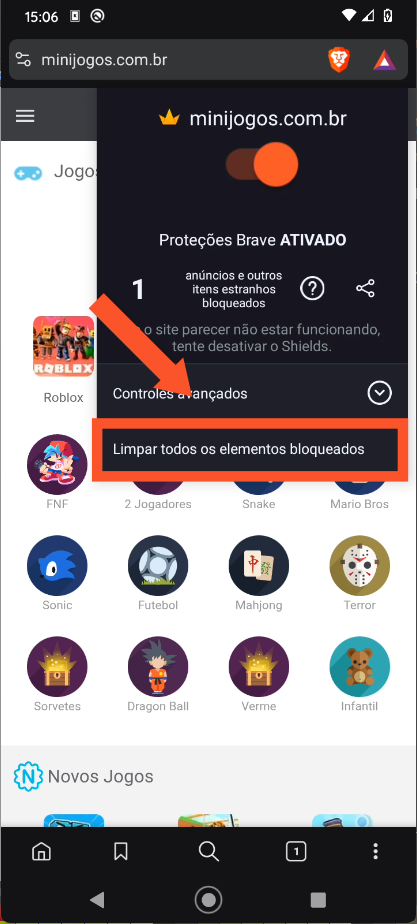
\includegraphics[trim={0cm 10cm 0cm 0cm}, clip, width=\textwidth]{imagens/brave_bloqueio_elementos_09.png}\\[0.2cm]
		\textbf{\textcolor{BraveOrange}{\faMobile* \ Passo 9}}
	\end{minipage}
	\hfill
	\begin{minipage}{0.45\textwidth}
		\centering
		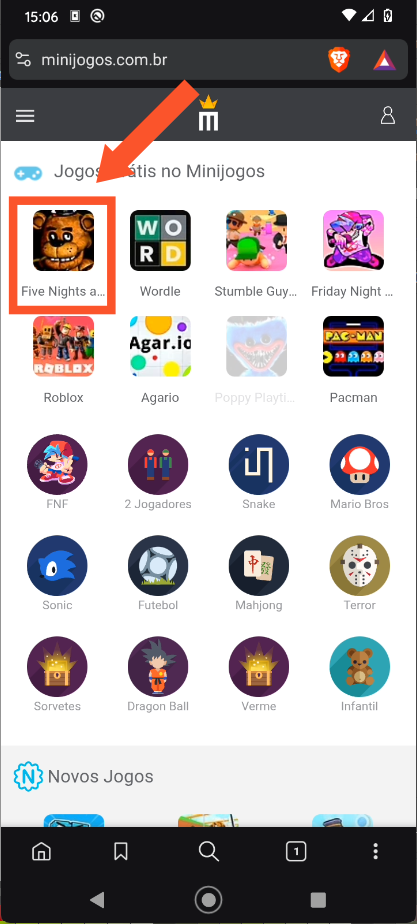
\includegraphics[trim={0cm 10cm 0cm 0cm}, clip, width=\textwidth]{imagens/brave_bloqueio_elementos_10.png}\\[0.2cm]
		\textbf{\textcolor{BraveOrange}{\faMobile* \ Passo 10}}
	\end{minipage}
\end{minipage}
% AdguardGreen

\vspace{0.5cm} % Respiro
\noindent
\begin{minipage}{\textwidth}
	\textcolor{BraveOrange}{\textbf{Passo 9:}} Toque em \enquote{Limpar todos os elementos bloqueados}\newline
	\textcolor{BraveOrange}{\textbf{Passo 10:}} Pronto, o elemento retornou para o loval de origem (retornou a ficar visível e disponível?).
\end{minipage}
\vspace{0.3cm}

Você também pode experimentar essa funcionalidade em qualquer rede social de sua preferência como o Facebook, TikTok, Instagram e etc. Fica meu forte incentivo para fazer esses experimentos.

Além disso, você também pode explorar as outras opções do menu suspenso, como:

\begin{itemize}
	\item \textbf{Fazer upgrade de conexões para HTTPS:} Acione a opção \enquote{Exigir que todas as conexões usem HTTPS}, pois dessa forma todas as suas conexão serão as mais seguras possíveis (revise essa afirmação, pois não tenho muita certeza)
	\item \textbf{Bloquear rastreadores e anúncios:} Aqui, a opção  Acione a opção \enquote{Bloquear rastreadores e anúncios (agressivo)} ativada resulta em uma página livre de propagandas. Teste no Facebook, por exemplo.
	\item \textbf{Bloquear cookies:} Essa opção deve ser usada com cautela, pois plataformas como o Facebook, podem te expulsar até que você desfaça essa ação. Então, caso essa expulsão ocorra, basta desfazer essa ação que volta todo ao normal.
	\item \textbf{Bloquear impressão digital:} Deixe como está, pois essa é a melhor forma de seu dispositivo ser menos assediado na Web.
\end{itemize} 

\begin{tcolorbox}[colback=NordBackground, colframe=BraveOrange, title=\faYoutube \ Dica de Ouro para as Mães]
	\textcolor{white}{Se você quiser deixar a criança assistindo a desenhos no celular sem o risco de aparecerem propagandas no meio do vídeo, basta abrir o site do YouTube diretamente \textbf{dentro} do navegador Brave. A mágica acontece na hora!}
\end{tcolorbox}